\section{Jenis Pembelajaran}
Ada beberapa jenis pembelajaran yang dimiliki oleh \emph{machine learing}, itu tergantung pada jenis data yang tersedia. Namun secara luas jenis pembelajaran
\emph{machine learning} terbagi menjadi tiga bagian, yaitu \emph{supervised learning}, \emph{unsupervised learning}, dan \emph{reinforcement learning}.
\subsection{Supervised Learning}
Supervised learning menjadi jenis \emph{machine learning} paling mendasar. Dalam konteks ini tujuan dari \emph{supervised learning} adalah
untuk memperoleh kemampuan menggeneralisasi, yang mengacu pada kemampuan bahwa hasil jawaban yang tepat dapat ditebak untuk pertanyaan yang tidak diajarkan.
Dengan demikian, pengguna tidak harus mengajarkan semuanya ke program, tetapi program dapat secara otomatis mengatasi situasi yang tidak diketahui dengan hanya mempelajari
sebagian kecil pengetahuan saja.

Algoritma yang tergolong \emph{supervised learning} biasanya digunakan untuk menyelesaikan berbagai persoalan yang berkaitan dengan:
\begin{itemize}
    \item  \emph{Classification} (Klasifikasi)

          \emph{Classification} dapat didefinisikan sebagai proses memprediksi kelas atau kategori dari nilai yang diamati
          atau titik data yang diberikan. Ada dua jenis tipe \emph{classification} yaitu \emph{Binary Classifier} dan \emph{Multi-class Classifier}.

          Secara matematis, \emph{classification} adalah tugas pemetaan fungsi $(f)$ dari variabel \emph{input} $(x)$ ke variabel \emph{output} $(y)$
          \begin{figure}[h]
              \centering
              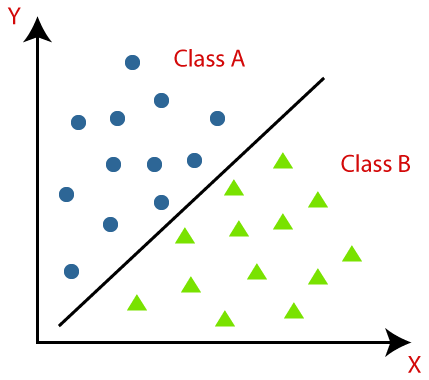
\includegraphics[scale=0.25]{classification-algorithm}
              \caption{Classification algorithm \cite{JavatpointClassificationAlgImage}}
          \end{figure}
    \item  \emph{Regression} (Regresi)

          \emph{Regression} dapat didefinisikan sebagai suatu metode analisis statistik yang digunakan agar dapat melihat pengaruh antara dua variabel atau lebih.
          Hubungan variabel yang dimaksud bersifat fungsional yang diwujudkan dalam bentuk model matematis.
          Pada analisis regresi, variabel dibagi menjadi dua jenis yaitu variabel respons atau biasa disebut variabel bergantung dan variabel bebas atau dikenal dengan istilah variabel independen.
          Ada beberapa jenis analisis regresi yaitu regresi sederhana meliputi regresi linier sederhana dan non-linier sederhana dan regresi berganda meliputi linier berganda atau non-linier berganda.
          \begin{figure}[h]
              \centering
              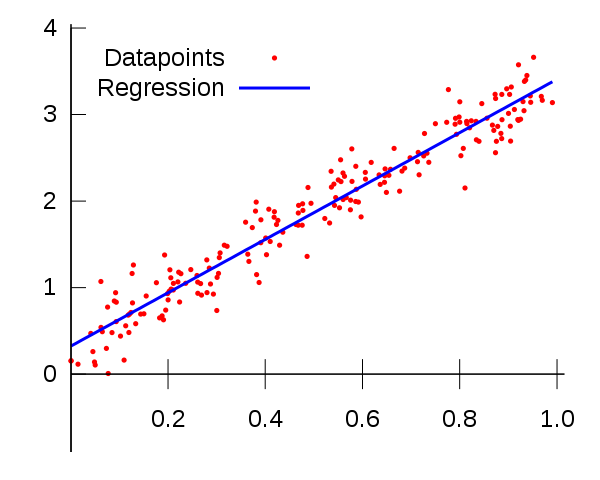
\includegraphics[scale=0.25]{regression-algorithm}
              \caption{Regression algorithm \cite{DavidFumoRegression}}
          \end{figure}
\end{itemize}
\subsection{Unsupervised Learning}
\emph{Unsupervised learning} mempertimbangkan situasi dimana tidak ada pengawasan dalam pembelajaran. Dalam konteks ini, program mengumpulkan data secara mendiri melalui internet dan mencoba mengekstrak pengetahuan yang bermanfaat tanpa bimbingan dari pengguna.
Konsep yang metode ini gunakan jauh berbeda dengan metode \emph{supervised learning} dimana pada metode ini hasil yang diharapkan tidak dapat diketahui oleh siapapun.
Dengan kata lain, hasil yang akan ditampilkan hanya bergantung kepada nilai bobot yang disusun pada awal pembangunan sistem dan tentu masih dalam ruang lingkup tertentu.

Contoh Studi Kasus pemecahan masalah dengan metode \emph{unsupervised learning} adalah misal suatu pusat perbelanjaan ingin melakukan bongkar muat terhadap satu truk berisi sepatu campur.
Agar dapat dijual sepatu-sepatu tersebut perlu dikelompokkan brand dan ukurannya.
Dalam hal ini, pihak pusat perbelanjaan tidak perlu memasukkan datanya terlebih dahulu karena data yang ada dilapangan saat itulah yang langsung diproses untuk mengelompokkan sepatu-sepatu tersebut sesuai brand dan ukurannya\cite{AlFahriz}.
\begin{figure}[h]
    \centering
    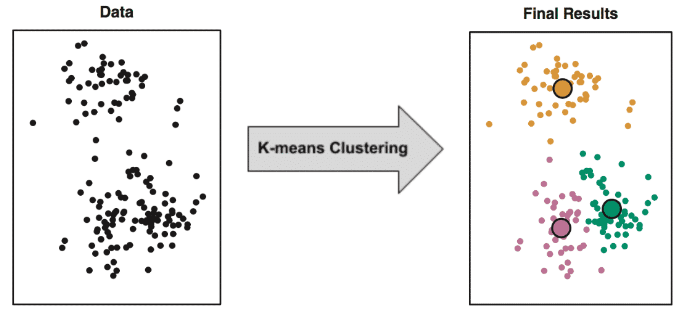
\includegraphics[scale=0.25]{unsupervised-learning}
    \caption{Unsupervised Learning \cite{AlFahriz}}
\end{figure}

\subsection{Reinforcement Learning}
\emph{Reinforcement learning} bertujuan untuk memperoleh kemampuan generalisasi dalam cara yang sama seperti \emph{supervised learning}.
Bedanya, \emph{supervisor} tidak memberikan solusi atau jawaban secara langsung. Sebaliknya, \emph{supervisor} hanya mengevaluasi perilaku program (agen) dan memberikan \emph{feedback}.
Dibandingkan dengan \emph{supervised learning}, \emph{reinforcement learning} berbeda dalam hal tujuan, dalam kasus \emph{reinforcement learning} tujuannya adalah untuk menemukan model tindakan yang sesuai yang akan memaksimalkan total \emph{cumulative reward} agen.
Dengan kata lain
\emph{reinforcement learning} adalah mempertimbangkan masalah dan mengarahkan
pada tujuan saat berinteraksi dengan lingkungan yang tidak pasti. Agen
menerima state(representasi dari enviroment) dan memilih action. Selanjutnya
agent akan menerima nilai reward dari action yang dipilih. Agen akan berusaha
memaksimalkan reward yang diterima dari waktu ke waktu.
\begin{figure}[h]
    \centering
    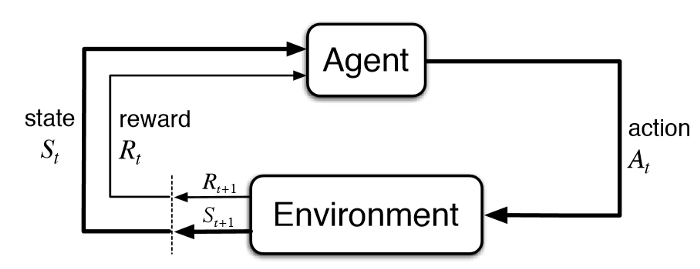
\includegraphics[scale=0.25]{reinforcement-learning}
    \caption{Reinforcement Learning \cite{TWDSReinforcementLearning}}
\end{figure}